\chapter{Privacidade}
\label{cap:privacidade}
% \chapter{Fundamentação teórica}
% \label{cap:fundamentacao}
% Mind Map para Fundamentação te: https://bit.ly/3P5rG3q

% Durante o estudo bibliográfico, foram lidos diversos artigos sobre a privacidade vs BC. O trabalho é organizar os artigos, criando um texto que convença o leitor de que eles são interligados e mostram cada ponto necessário para a resolução do problema, o objetivo e a justificativa vão ser incluídos posteriormente.

% Lembrar de mencionar que DLT e BC são intercambiáveis. Adicionar as siglas na seção de acronismos.

% Contextualização: Qual o papel da privacidade na sociedade moderna? Como atingir a privacidade em ambientes abertos e inseguros? Uma discussão sobre a influência da GDPR no Blockchain.

Privacidade e proteção de dados são duas questões inter-relacionadas de governança da Internet. A proteção de dados é um mecanismo legal que garante a privacidade. A privacidade é geralmente definida como o direito de qualquer cidadão de controlar suas próprias informações pessoais e decidir sobre elas (divulgar informações ou não). A privacidade é um direito humano fundamental. É reconhecido na Declaração Universal dos Direitos Humanos, no Pacto Internacional sobre Direitos Civis e Políticos e em muitas outras convenções internacionais e regionais de direitos humanos \cite{PrivacyA6:online}. 

A diferença entre privacidade e proteção de dados, segundo Guamán \cite{Privacyv4:online}, depende do país e das idiossincrasias da língua falada. Nos Estados Unidos da América (United States of America - USA), o termo privacidade domina as regras e práticas de processamento de dados pessoais, na União Européia (European Union - EU) o termo proteção de dados parece ser utilizado para se referir a mesma definição. Para evitar problemas de linguagem e suas diferenças, a EU utiliza o termo proteção de dados ao invés de privacidade para se referir a proteção da privacidade proteção do direito de privacidade no que diz respeito ao tratamento de dados pessoais.

Na segurança de dados os termos dados pessoais, informações pessoais ou Informações de Identificação Pessoal (Personally Identifiable Information - PII) são usados para descrever informações que podem ser usadas para identificar, contactar e localizar uma pessoa \cite{Personal37:online}. Dentro do tema privacidade, esta tese preocupa-se na privacidade dos dados pessoais, proteção dos dados, por isso os termos privacidade, proteção de dados e PII são intercambiáveis.

% No trabalho de Schwerin2018 menciona-se que PII e privacidade são termos intercambiáveis. Estou procurando uma forma de adicionar essa idéia na tese.

Segundo \citet{Schwerin2018} a definição de PII muda com o desenvolvimento de tecnologias como blockchain, IA, Big Data e Internet das coisas (Internet of Things - IoT), pois aumentam a chance de reidentificar os dados. %apud 16.
Quase todos os dispositivos digitais usados por humanos e conectados à internet podem ser usados para rastrear sua origem. %(apud [17]).
Como esse tipo de dado está frequentemente ligado à identidade de um ser humano, ele deve ser protegido da mesma forma que outros direitos que esse indivíduo possui.

O aumento da coleta de dados pessoais pelas organizações trouxe riscos e desafios a segurança \citep{Teixeira2019:article}. Em 2012 o conselho da união européia começa a trabalhar na regulamentação EU 2016/679, entrando em vigor em 25 de maio de 2018. Segundo \citet{gabriela_eu_2018:article} e \citet{Teixeira2019:article}, a nova lei revoga as diretrizes 95/46/EC, conhecida como a norma de proteção de dados da UE (EU Data Protection Directive). Com a intenção de dar mais controle aos cidadãos sobre seus dados pessoais, a GDPR impõe um conjunto de obrigações em respeito a guarda, processamento, coleta e divulgação de dados. A regulação é válida para qualquer organização que processe os dados e prevê multas pesadas quando a não conformidade com as regras são detectadas \citep{EuropeanCommission2016:misc}.

Nesse contexto as empresas e governos fazem o papel de concentradores de dados, onde os usuários possuem um controle limitado sobre suas informações. As SNS (Social Network Sites) estão no foco principal, pois seus usuários disponibilizam uma grande quantidade de informações pessoas para esses sites. Para gerar modelos de negócios, essas organizações armazenam, distribuem, analisam informações confidenciais de PII de seus usuários \cite{Al-ZabenNasr2018:article}. Em abril de 2018, veio a público o caso da Cambridge Analytica, onde 50 milhões de perfis de usuários do Facebook foram violados. Apontado como o maior vazamento de dados pessoais até aquele momento foram usados para criar ferramentas que direcionavam propagandas baseadas nos perfis coletados no Facebook, com o objetivo de influenciar as eleições americanas em 2015.

%e plataformas afins fazem a coleta de dados de PII \citep{Al-ZabenNasr2018:article}. Em busca de um ambiente mais aberto, a tecnologia BC ou DLT vem direcionar o direito de uso da PII para o usuário, assim como está definido na GDPR. Em contrapartida contra a centralização de dados, o BC é uma resposta.... 

Para contrapor a grande concentração de dados de SNS --- temos tecnologias descentralizadas como o Blockchain. temos algumas respostas, como o Blockchain \citep{Schwerin2018}.

Para restaurar a confiança no mundo digital, uma solução proposta é a tecnologia Blockchain (abreviação BC) \citep{Schwerin2018}. Inicialmente a tecnologia foi desenvolvida para gerar transparência em transações financeiras envolvendo a criptomoeda Bitcoin \citep{Nakamoto2009}. Ultimamente a tecnologia tem ganho atenção de pesquisadores que vão além das transações financeiras envolvendo criptoativos \citep{Al-ZabenNasr2018:article}.

\textit{Parágrafo rascunho:} 
O Big data parece ter sido o motivador de tais ações de proteção de dados. A forma como empresas tem usado os dados de seus usuários, por centralizar essas informações em seus servidores. Sem fiscalização. Aprendizado de máquina sem o consentimento explicito do usuário. 

% Não esquecer de mencionar a parte de segurança da DLT.
\textit{Parágrafo rascunho:} 
Em contrapartida contra a centralização do dados, temos o BC \citep{Nakamoto2009}, que inicialmente foi uma tecnologia utilizada para gerar transparência no Bitcoin. Logo encontrou outros usos, permitindo que a confiança seja distribuída, retornando o controle da identidade ao próprio usuário. Mesmo assim a DLT encontra problemas próprios, como a identificação de um usuário. Trabalhos como XXX, XXX, XXX e XXXX falam dos problemas e soluções para o uso da DLT na era da GDPR e afins.

% Podemos falar da privacidade na DLT.

% Tecnologias AI, Big Data, IoT e BC. Grandes empresas centralizadora de PII Google, Facebook. Devido aos problemas de segurança e mal uso de dados, mostrar fontes. Estarão os usuário dispostos a continuar confiando no governo e nas empresas fornecedoras de serviços, seus dados para serem executados  Para trazer a confiança ao mundo

% BC é uma tecnologia que chegou para ficar, dados escritos são imutáveis e a prova de fraudes. Mas é um risco ao PII/Privacidade do usuário, que pode ser utilizado de maneira "evil" (ver nos artigos, existe uma forma melhor de referir-se ao abuso de dados, normalmente praticado por empresas) por indivíduos ou empresas.

Direito a privacidade na Blockchain. Como proteger os dados pessoais tem se tornado um tema cada vez mais importante \citep{Schwerin2018}. Uma preocupação crescente com o uso feito dos dados por grandes corporações. \cite{dsguaman} 
%[6]Privacy vs Data protection vs Information Security}. 
Se o BC (Blockchain) precisa estar em compliance com a GDPR, pergunta: é possível? Se sim, o que precisa ser feito?


No ecossistema da BC \cite{Schwerin2018} menciona sobre a evolução e mudança de paradigma que irá influenciar cada fragmento do mundo que conhecemos, apud [10].

Estratégias para proteger a privacidade. Segundo Hassan em seu artigo \cite{Hassan2020} a encriptação é uma das maneiras tradicionais de proteger a privacidade usada pela maioria dos sistemas para proteger os dados contra adversários e usuários não autorizados. Outra técnica é a anonimização de dados, que apud [23] \cite{Hassan2020} mostra que pode ser facilmente comprometidos. \cite{Dwork2006} propõe um trabalho que ao perturbar os dados, utilizando um processo de randomização, chamado Randomized Response proposto por S. L. Warner em 1965, a privacidade é alcançada através da negação plausível para qualquer entrada.

Esse processo tem sido utilizado em sistemas onde não se conhece a capacidade de processamento do hardware.

% Falar da GDPR. Contar um pouco da história. Verificar os artigos de referência se algum deles tem essa informação. Acho que o Schwerin2018 tem alguma informação relevante. Abaixo é uma explicação do site da UE.

A GDPR (General Data Protection Regulation) legisla como dados pessoais precisam ser coletados, processados e apagados. Entre os direitos que se destacam na lei, encontra-se o direito ao esquecimento \cite{Everythi34:online}.

De acordo com Al-Zaben \cite{Al-ZabenNasr2018:article}, um número significativo de usuários fazem uso de redes sociais, fornecendo uma grande quantidade de PII para sites e aplicativos de redes sociais. Ainda afirma que o BC ganhou muita atenção de vários pesquisadores(incluir apuds? [7] [8]). Com a inclusão da GDPR os dados individuais precisam ser protegidos, ficando as instituições obrigadas a recolher o consentimento individual de cada usuário para coletar e compartilhar seus dados. Ainda é necessário a empresa garantir que seus dados possam ser removidos de sua base, conhecido como ``direito ao esquecimento"". Propõe-se a criação de um BC capaz de gerenciar PII utilizando organizações. Separando a persistência de PII de outros dados.

Feng, no survey \cite{Feng2019} sobre proteção da privacidade no BC. Afirma que o BC é uma tecnologia disruptiva que funciona de maneira descentralizada. Sendo a tecnologia base para moedas digitais, como Bitcoin, operando de maneira distribuída sem o uso de uma entidade central.

% Parágrafo pode ir na seção de Blockchain - foco em IoT.
% Feng menciona o uso da tecnologia BC em IoT, por ser equipada com uma topologia descentralizada. O gerenciamento de equipamentos pode ser automatizado e a sincronização de dados pode ser fácil e rápida entre dispositivos IoT (Hud et al, 2017; Dorri et al. 2016; Conoscenti et al., 2016). Além disso o BC melhora a transparência e rastreabilidade de propriedade "Supply Chain Management Systems" (traduzir para o português) (várias referências). Além disso, a característica descentralizada do BC pode diminuir a pressão sobre servidores centralizados, para gerenciar infraestruturas de chaves públicas ou gerenciamento de sistemas de identidades (várias referências). Como contribuição apresenta uma análise crítica sobre mecanismos de defesa da privacidade no BC. 1) Definindo a privacidade além do usuário, incluindo a privacidade da transação. 2) Introduzindo ameaças existentes tanto para o usuário quanto para a transação no BC. 3) Introduzindo diversas tecnologias, especialmente técnicas de criptografia, que são usadas para proteger a privacidade no BC. 4) Os pontos para enteder a origem, objetivo e drawback de cada approach de proteção. 5) Avaliando o impacto de vários métodos para preservar a privacidade, em diversos protocolos em uso.

Do ponto de vista de \cite{Schwerin2018} mostra que os especialistas que responderam aos seus questionamentos no seu estudo "delphi", que o BC não deve capturar dados pessoais de seus usuários. Feng apresenta mecanismos de privacidade, incluindo a criptografia. % Melhorar esse parágrafo, adicionar outros autores que apontam para soluções off-chain. Talvez a LGPD, tem um artigo do Teixeira, que menciona algo nesse sentido.

% Identificar trabalhos que apontam soluções para gravar dados "off-chain", apontar para as referências. O objetivo disso é mostrar o esforço que esses pesquisadores tem em relação a compliance com a LGPD e GDPR.

% Currently,  over  50  million  people  use  several   Social   Networking   Sites   (SNS)   and   have   made   available  a  vast  amount  of  PII  on  these  sites.  All  these  SNS  sites, other websites and mobile applications offer sign in or registration  for  premium  services.  PII  are  often  utilized  by  organizations  to  authenticate  a  customer’s  identity.  Since  most of these SNS sites and applications are for free, several studies found PII breaching by these organizations. Actually, these  organizations  store,  distribute,  analyse  sensitive  PII  information in order to generate business model through user profiling.  Tech  giants  uses  third  party  service  providing \cite{Al-ZabenNasr2018:article}

\cite{article:BegumSNausheenF2018} Segurança dos Dados e Privacidade. Segundo Begum e Nausheen \cite{article:BegumSNausheenF2018}, segurança dos dados é comumente conhecida como confidencialidade, disponibilidade e integridade dos dados, garantindo que os dados não sejam usados por usuários não autorizados. Um plano de segurança de dados inclui apenas coletar as informações necessárias, mantê-las seguras e destruir qualquer informação que não seja mais necessária. Ainda, a privacidade dos dados é definida como o uso apropriado dos dados. Quando empresas e comerciantes usam dados ou informações que lhe são fornecidos, os dados devem ser usados de acordo com os fins acordados, sem divulgar as informações do consumidor. As abordagens para alcançar a privacidade são: encriptação, inclusão de ruídos e anonimização.

% Aqui abrimos para expandir cada um dos assuntos.

\chapter{Mecanismos de Privacidade}
Begum \cite{article:BegumSNausheenF2018}.

\chapter{Privacidade Diferencial}
\label{cap:privacidadediferencial}

\chapter{Privacidade no Blockchain}
\label{cap:blockchain}
Feng \cite{Feng2019}.

\section{Privacidade Diferencial no Blockchain}
Hassam \cite{Hassan2020}. % Deveria ser o survey.

\chapter{Alguns exemplos}
\label{cap:exemplos}

% figuras estão no subdiretório "figuras/" dentro deste capítulo
\graphicspath{\currfiledir/figuras/}

%=====================================================

\section{Guias de \LaTeX}

Este modelo contém exemplos para os padrões de inserção de figuras, tabelas, listas de itens, bibliografia, etc. Em caso de dúvidas ou discordância, Pode-se entrar em contato com a direção ou secretaria do programa. Obviamente, críticas (construtivas) e sugestões são muito bem-vindas.

Para aprender a usar \LaTeX, um bom guia introdutório disponível na Internet é \cite{oetiker07}, que também tem uma versão em português. Para tópicos mais avançados consulte \cite{goossens93}.

%=====================================================

\section{Estrutura do texto}

Para melhorar a legibilidade do texto, deve ser evitado o uso de subdivisões mais profundas que a subseção (por exemplo, subsubseções). Se elas forem absolutamente necessárias, não devem ser numeradas. Deve-se analisar a possibilidade de uso de uma lista de itens em seu lugar. O número de níveis de texto do documento não deve exceder três: capítulo, seção e subseção. O uso de mais que três níveis dificulta a leitura e prejudica muito a estética do texto.

%=====================================================

\section{Estilo de redação}

Ao elaborar o texto da dissertação ou da tese, o mais indicado é o uso do verbo na forma impessoal. Exemplos:

\begin{itemize}
\item ... utilizaram-se os seguintes dados ...
\item ... elaborou-se de forma precisa ...
\item ... trata-se os algoritmos ...
\item ... foram obtidos resultados significativos ...
\end{itemize}

Além disso, deve-se a todo custo evitar a ``linguagem de revista'', com expressões como ``sensacional'', ``impressionante'', ``monstruoso'', etc (por exemplo: ``Os resultados obtidos são sensacionais, sobretudo considerando a monstruosa margem de erro.'').

%=====================================================

\section{Alguns exemplos}

Esta seção traz algus exemplos de elementos típicos de um texto científico, como figuras, tabelas e fórmulas matemáticas.

%=====================================================

\subsection{Exemplo de figura}

A forma sugerida para incluir figuras em um documento \LaTeX\ é importá-las usando o pacote \texttt{graphicx}. Como formatos gráficos sugere-se:

\begin{itemize}

\item Formatos \emph{raster}, como PNG (\emph{Portable Network Graphics}) ou JPG (\emph{Joint Photographic Experts Group}) para fotografias; procure usar uma resolução de ao menos 150 dpi (\emph{dots per inch}).

\item Formatos vetoriais, como PDF (\emph{Portable Document Format}) ou EPS (\emph{Extended PostScript}) para diagramas e gráficos\footnote{NUNCA use JPG ou GIF para desenhos vetoriais, pois o resultado final geralmente fica borrado.}.

\end{itemize}

A maior parte das ferramentas permite exportar figuras nesses formatos (a figura do exemplo foi produzida com o \emph{Inkscape}, um programa livre multiplataforma). A figura \ref{fig:comun-intra-inter} mostra um exemplo de inclusão de figura em PDF.

% exemplo de inserção de figura
\begin{figure}[!htb]
\centering
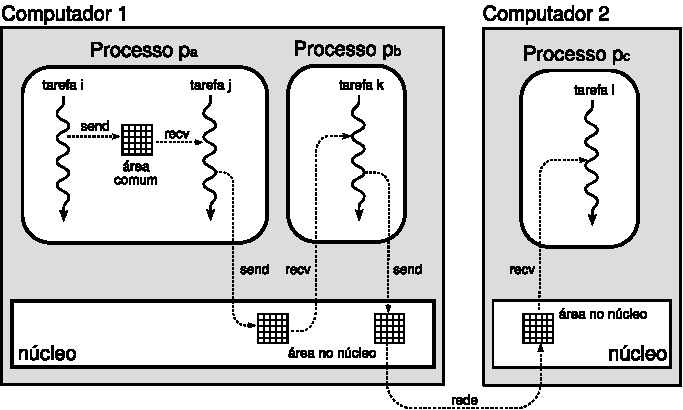
\includegraphics[width=12cm]{exemplo-figura.pdf}
\caption{Comunicação inter-processos.}
\label{fig:comun-intra-inter}
\end{figure}

Para mais informações consulte \cite{goossens93}.

%=====================================================

\subsection{Exemplo de tabela}

Tabelas são elementos importantes de um documento. No \LaTeX\ as tabelas podem ser objetos flutuantes (definidas no ambiente \texttt{table} e referenciadas por números usando \texttt{label} e \texttt{ref}) ou objetos fixos simples, criados pelo ambiente \texttt{tabular}. A tabela \ref{tab:modelos} é um exemplo de tabela flutuante, cuja posição no texto pode variar em função das quebras de página.

\begin{table}[!htp]
\centering
\caption{Os 16 modelos centrais do UCON$_{\mathrm{ABC}}$}
\label{tab:modelos}
\begin{tabular}{|c|cccc|}
\cline{2-5}
\multicolumn{1}{c|}{}& 0 (imutável) & 1 (\emph{pre-update}) & 2 (\emph{on-update}) & 3 (\emph{pos-update}) \\
\hline
\texttt{preA} & \textbullet & \textbullet & -- & \textbullet \\
\hline
\texttt{onA} & \textbullet & \textbullet & \textbullet & \textbullet \\
\hline
\texttt{preB} & \textbullet & \textbullet & -- & \textbullet \\
\hline
\texttt{onB} & \textbullet & \textbullet & \textbullet & \textbullet \\
\hline
\texttt{preC} & \textbullet & -- & -- & -- \\
\hline
\texttt{onC} & \textbullet & -- & -- & -- \\
\hline
\end{tabular}
\end{table}

%=====================================================

\subsection{Exemplo de fórmula}

Equações destacadas devem ser numeradas como mostra a equação \ref{eq:relatividade}:

\begin{equation}
E = m \times c^2
\label{eq:relatividade}
\end{equation}

%=====================================================

\subsection{Exemplos de código-fonte}

Códigos-fonte podem ser produzidos de forma simples através do ambiente \texttt{verbatim}, como mostra este exemplo:

\begin{footnotesize}
\begin{verbatim}
#include <stdio.h>

int main (int argc, char *argv[])
{
   int i ;                           // uma variavel local

   for (i=0; i< 100; i++)            // um laço for
      printf ("i vale %d\n", i) ;    // uma saída na tela
}
\end{verbatim}
\end{footnotesize}

No entanto, é preferível usar pacotes especializados para a edição ou inclusão de códigos-fonte, como o pacote \texttt{listings}. Eis um exemplo de código-fonte escrito com esse pacote:

% exemplo de código-fonte definido no próprio texto

\begin{lstlisting}
#include <stdio.h>

int main (int argc, char *argv[])
{
   int i ;                           // uma variável local

   for (i=0; i< 100; i++)            // um laço for
      printf ("i vale %d\n", i) ;    // uma saída na tela
}
\end{lstlisting}

Esse pacote também permite incluir códigos-fonte de arquivos externos. Eis um exemplo:

% exemplo de código-fonte incluso

\lstinputlisting{2-fundam/exemplo.c}

%=====================================================

\subsection{Exemplo de algoritmo}

Os pacotes \texttt{algorithm} e \texttt{algorithmic} permitem formatar algoritmos facilmente. Eis um exemplo:

\begin{algorithm}[H]
\caption{Ações de $s_i$ ao encerrar um ciclo:}
\label{alg:on-period-ending}
\begin{small}
\begin{algorithmic}[1]
\FORALL{$x \in \mathcal{K}_i$}
  \STATE{$\mathit{banned}_i(x) \gets$ FALSE}
  \STATE{$mi_i(x) \gets 0$}
  \STATE{$mm_i(x) \gets 0$}
  \STATE{$\mathit{age}_i(x) \gets \mathit{age}_i(x) + 1$}
  \IF{$\mathit{age}_i(x) = \mathit{age}_\mathit{max}$}
     \STATE{$\mathcal{K}_i \gets \mathcal{K}_i - \{x\}$}
     \COMMENT{``esquece'' do servidor $x$}
     \STATE{remove as informações locais sobre $x$}
     \STATE{envia $\mathit{notify}(x,\mathit{undef})$ ao grupo de confiança $\mathcal{T}_i$}
  \ENDIF
\ENDFOR
\end{algorithmic}
\end{small}
\end{algorithm}
 
%=====================================================

\subsection{Exemplo de citação}

Como afirmou Maquiavel em seu livro \emph{O Príncipe}:

\begin{quote}
``Nada é mais difícil de instituir, mais perigoso de conduzir, mais incerto no seu sucesso, do que liderar a introdução de uma nova ordem de coisas... O inovador faz inimigos em todos aqueles que prosperavam sobre as antigas regras, e somente tíbio suporte é esperado daqueles que prosperariam na novidade, porque os homens são geralmente incrédulos, nunca realmente confiam nas coisas novas, a menos que as tenham testado em experiência''.
\end{quote}

%=====================================================

\section{Uma seção}

\subsection{Uma subseção}

\subsubsection{Uma subsubseção}

%=====================================================

\section{Conclusão}

Todo capítulo (com exceção da introdução e da conclusão) deve encerrar com uma pequena conclusão local, resumindo os tópicos apresentados no capítulo e preparando o leitor para o próximo capítulo (exceto se esse for a conclusão geral). Caso o capítulo tenha apresentado resultados obtidos pelo próprio autor, estes devem ser sucintamente relembrados aqui.

%=====================================================
